\documentclass{beamer}
\usepackage[spanish,activeacute]{babel}
\usepackage[utf8]{inputenc}
\usepackage{verbatim}
\usepackage{color}
\usepackage{alltt}


\definecolor{gray2}{rgb}{100,100,100}
\definecolor{red}{rgb}{255,0,0}
\definecolor{green}{rgb}{0,1,0} 
\definecolor{blue}{rgb}{0,0,1} 
\newcommand{\blue}{\textcolor{blue}}
\newcommand{\red}{\textcolor{red}}
\newcommand{\green}{\textcolor{green}}

\usetheme[pageofpages=of,% String used between the current page and the
                         % total page count.
          alternativetitlepage=true,% Use the fancy title page.
          titlepagelogo=img/1,% Logo for the first page.
          watermark=,% Watermark used in every page.
          watermarkheight=150px,% Height of the watermark.
          watermarkheightmult=4,% The watermark image is 4 times bigger
                                % than watermarkheight.
          ]{Torino}

\usecolortheme{nouvelle}

\author{\large Cristián D. Maureira Fredes}
\title{\huge Car Sequencing Problem}
\subtitle{\large \textit{``Una aproximación utilizando Selección Clonal''}}
\institute{\textbf{Taller de Métodos y Modelos Cuantitativos}\\ Departamento de Informática\\ (UTFSM)}
\date{\today}

\begin{document}

\begin{frame}[t,plain]
\titlepage
\end{frame}


\section{Introducción}
Una expresión regular,
a menudo llamada también patrón,
es una expresión que describe un conjunto de cadenas sin enumerar sus elementos.

Además,
normalmente representan otro grupo de caracteres mayor,
de tal forma que podemos comparar el patrón con otro conjunto de caracteres para ver las coincidencias.

La mayoría de las formalizaciones proporcionan los siguientes constructores:
una expresión regular es una forma de representar a los lenguajes regulares
(finitos o infinitos) y se construye utilizando caracteres del alfabeto
sobre el cual se define el lenguaje.

Específicamente,
las expresiones regulares se construyen utilizando los operadores
unión, concatenación y clausura de Kleene.

Las expresiones regulares en UNIX (RE's) están recogidas en el estándar POSIX 1003.2.



\section{Definición del Problema}
%Descripción del problema, su complejidad, en que consiste, cuales son sus objetivos,
%restricciones, variantes más conocidas. 

El \emph{Car Sequencing Problem} es un problema de satisfacción de restricciones (CSP), posee la
característica de ser NP-duro~\footnote{
NP-duro es el conjunto de los problemas de decisión que contiene los problemas H
tales que todo problema L en NP puede ser transformado polinomialmente en H.
Esta clase puede ser descrita como conteniendo los problemas de decisión que son
al menos tan difíciles como un problema de NP.}
, además corresponde a un tipo de variación del problema NP-completo \emph{Job-Shop Scheduling}.%,
%pero con un uso de razonamiento automatizado, es decir, con un enfoque dedicado a estudiar y comprender
%diferentes características del razonamiento, permitiendo así construir programas que le den la posibilidad
%a los computadores para razonar en forma autónoma.
 
Siguiendo la misma idea, es válido señalar que el \emph{Car Sequencing Problem} es un tipo de problema de planificación
de tareas en una línea de ensamblaje de autos, donde cada uno es perteneciente a un clase de automóvil, debido al conjunto
de opciones y accesorios que posee (airo acondicionado, centralizado eléctrico, etc), y cada una de las opciones o
accesorios se instala en una planta distinta, por lo que el objetivo principal es el poder encontrar el orden en la
secuencia de los vehículos, preocupándonos de no exceder la capacidad de cada planta de ensamblaje y también cumplir con la demanda.

Por lo tanto, si realizamos una definición más formal de nuestro problema, podríamos decir lo siguiente:
Teniendo una lista de vehículos dada, cada uno con sus respectivas opciones requeridas,
necesitamos establecer un orden en la línea de ensamblaje, con el fin de que cada subsecuencia de $q$ vehículos
tengamos a lo más $p$ que requieren de una determinada opción. Es importante tener en consideración que los
valores de $p$ y $q$ están asociados a cada opción de los vehículos.

Con respecto a la información que el problema otorga, podemos decir que contamos con:
\begin{itemize}
	\item Cantidad de vehículos de cada tipo o clase a producir (demanda)
	\item Lista de las opciones con la cual se constituye cada tipo o clase de vehículo, la cual puede utilizar una representación
		booleana para saber si cierto tipo de automóvil posee o no una determinada opción.
	\item Capacidad de las plantas que se preocupan de instalar la determinada opción.
\end{itemize}

Nuestro objetivo principal es:
\begin{itemize}
	\item Encontrar un orden en nuestra secuencia, que sirva para minimizar el costo por cada restricción insatisfecha.
\end{itemize}

Con respecto a las restricciones, tenemos que:
\begin{itemize}
	\item En cada subsecuencia de los $q$ vehículos, a lo más pueden haber $p$ que requieran de la opción determinada.
		Donde $p$ y $q$ son valores asociados a cada opción.
	\item La capacidad de cada planta de ensamblaje no puede ser excedida, es decir, cumplir con la demanda de cada automóvil
		sin abusar de una planta determinada.
	\item Por cada tipo de auto, el numero de autos de ese tipo debe ser secuenciado, es decir, todos los automóviles de cada clase
		deben estar presente en una secuencia determinada.
\end{itemize}





\subsection{Estado del arte problema}
%En que nivel se ha investigado la técnica aplicada al problema
%     (existe o no investigación, cuantas, cuales modelos, componentes
%     de la técnica, como es su desempeño, etc.).
%     En caso de no existir investigación o si a usted le parece que es
%     un aporte, experiencias con problemas similares o que podría ser útil
%     para su trabajo.

%existe o no?
%experiencias similares
\frame
{
\frametitle{Estado del Arte}
\framesubtitle{Existencia del acercamiento}
\begin{itemize}
	\item Actualmente en las grandes fuentes de publicaciones, como lo son:
	\begin{itemize}
		\item ACM.
		\item Springerlink.
		\item IEEE.
		\item Google Scholar.
	\end{itemize}
	\item \textbf{NO} existe un acercamiento utilizando \emph{Clonal Selection}
		para la resolución del \emph{Car Sequencing Problem}.
	\item Estado del arte del \emph{ROADEF}.
\end{itemize}
}

\frame
{
\frametitle{Estado del Arte}
\framesubtitle{Experiencias Similares}
\begin{block}{Mobile Robot Path Planning}
\begin{itemize}
	\item Operadores Inmunes:
	 \begin{itemize}
	 	\item \emph{Operador de Mutación:}
			consiste en elegir aleatoreamente un nodo del camino y \textbf{reemplazarlo} por otro nodo que no esté en el camino original. (intercambio de opciones válidas)
		\item \emph{Operador de Inserción:}
			se utiliza para poder \textbf{reparar} los segmentos de un camino infactible, insertando un nodo entre el problema. (cambiar el elemento inválido por otro)
		\item \emph{Operador de Supresión:}
			se aplica a los caminos factibles e infactibles, para \textbf{disminuir costos}. (formas de disminuir el fitness por orden)
	 \end{itemize}
\end{itemize}
\end{block}
}

\frame
{
\frametitle{Estado del Arte}
\framesubtitle{Experiencias Similares}
\begin{block}{Scheduling Aircraft Landing}
\begin{itemize}
	\item Basar la selección clonal en:
	\begin{itemize}
		\item \emph{Infeasibility Degree (IFD):}
			maneja las restricciones de una buena manera y guía el proceso de optimización de manera efectiva.
		\item \emph{Excellent Gene Segment Spread (EGSS):}
			mejora la velocidad de convergencia del algoritmo.
	\end{itemize}
\end{itemize}
\end{block}
}

\frame
{
\frametitle{Estado del Arte}
\framesubtitle{Experiencias Similares}
\begin{block}{Vehicle Routing Problem}
\begin{itemize}
	\item Operadores de Mutación:
	\begin{itemize}
		\item \emph{EXC:}
			elige \textbf{esquinas} del camino y las trata de \textbf{unir}. (no sirve mucho)
		\item \emph{SUM:}
			que intenta \textbf{concatenar} dos rutas sin violar restricciones. (tipo de cruzamiento en un punto)
		\item \emph{NEW:}
			que \textbf{construye} nuevas ruta utilizando la heurística greedy a partir de un vértice aleatorio. (mejorar individuos particulares)
	\end{itemize}
\end{itemize}
\end{block}
}

\frame
{
\frametitle{Estado del Arte}
\framesubtitle{Experiencias Similares}
\begin{block}{Job-shop scheduling problem}
\begin{itemize}
	\item Variar la función objetivo en caso de encontrar mínimos locales, para escapar de los \emph{óptimos locales}.
	\begin{itemize}
		\item Primero, aumenta la función objetivo para hacer desaparecer los mínimos locales. (sumándole un factor con constantes positivas)
		\item Segundo, estira el vecindario de la variable auxiliar. (del paso anterior)
	\end{itemize}
\end{itemize}
\end{block}
}

\frame
{
\frametitle{Estado del Arte}
\framesubtitle{Experiencias Similares}
\begin{block}{Parallel Graph Coloring Problem}
\begin{itemize}
	\item Inicializar anticuerpos de forma aleatoria o utilizando \emph{greedy}.
	\item Utilizar conceptos de paralelismo.
	\item Concepto de \emph{migración}.
\end{itemize}
\end{block}
}


\section{Descripción de la Técnica}
%Origen de la técnica, descripción de la metáfora, componentes, modelos que existen etc.
\subsection{Origen biológico}

El principio de selección clonal es un modelo que explica la forma en la cual el sistema inmune
responde a una determinada infección y como algunos tipos de linfocitos T y B son seleccionados
para destruir un determinado antígeno que está invadiendo el cuerpo del sujeto.

Fue propuesto por el virólogo australiano, Sir Frank Macfarlane Burnet en el año 1959,
con un trabajo titulado \emph{``The clonal selection theory of acquired immunity''}.

Existen cuatro postulados fundamentales en la hipótesis de la selección clonal, los cuales son detallados más adelante:
\begin{enumerate}
	\item Cada linfocito soporta un solo tipo de receptor con una única especificación.
	\item La ocupación del receptor es requerida para la activación de la célula.
	\item Las células efectoras diferenciadas derivadas desde un linfocito activado soportarán receptores de una especificación idéntica al de la célula padre.
	\item Aquellos linfocitos que soportan receptores para moléculas propias serán eliminados en una etapa temprana.
\end{enumerate}

%[[
%The clonal selection theory is proposed by Burnet in 1978, the main features of which are summarized as following [8]:
%(1) The new cells are copies of their parents (clone) subjected to a mutation mechanism with high rates (somatic hyper-mutation);
%(2) Elimination of newly differentiated lymphocytes carrying self-reactive receptors;
%(3) Proliferation and differentiation on contact of mature cells with antigens;
%(4) The persistence of forbidden clones, resistant to early elimination by self-antigens, as the basis of autoimmune diseases.
%]]

De acuerdo a la teoría propuesta por Burnet, el repertorio del sistema inmune se somete a un mecanismo de selección durante el tiempo de vida de un individuo.
La teoría establece que al unirse con un antígeno adecuado, se produce la activación de los linfocitos.
Una vez activado, los clones de los linfocitos son producidos con receptores idénticos a los linfocitos originales que encontraron el antígeno.
Así ocurre una expansión clonal de los linfocitos originales.
Esto asegura que solo los linfocitos específicos que se han activado gracias a un antígeno sean producidos en grandes cantidades.
La teoría de la selección clonal también establece que cualquier linfocito que tenga receptores de antígenos de moléculas propias del organismo
debe ser eliminada durante el desarrollo de los linfocitos.
Esto asegura que solo los antígenos de un patógeno pueden causar que un linfocito se clone y se expanda y así generar una respuesta inmune adaptativa a
agentes externos.
Durante la expansión clonal de linfocitos B, el promedio de la afinidad entre los anticuerpos aumenta para el antígeno que desencadena la expansión clonal.
Este fenómeno se llama maduración de la afinidad, y es responsable de el hecho de que en una posterior exposición al antígeno, la respuesta inmune es más eficaz debido a los anticuerpos con una mayor afinidad por el antígeno.
La maduración de la afinidad es causada por una hiper-mutación somática y un mecanismo de selección que ocurre durante la expansión clonal de linfocitos B.
La hiper-mutación somática altera la especificación de los anticuerpos, introduciendo cambios aleatorios a los genes que lo forman.
\begin{figure}[h!]
\begin{center}
\includegraphics[width=0.5\textwidth]{img/clonalSelection.pdf}
\end{center}
\caption{Ejemplo de una selección clonal de linfocitos}
\label{fig:clonalSelection}
\end{figure}

Se señala la descripción de la figura~\ref{fig:clonalSelection} se detalla a continuación:

La teoría de la selección clonal de los anticuerpos indica que un linfocito B immaduro
se activa frente a la exposición de los antígenos, su posterior diferenciación en células
plasmáticas que sintetizan anticuerpos específicos en contra del antígeno y células de memoria.


\subsection{Algoritmo de la Selección Clonal}

Siguiendo el principio de selección clonal y el proceso de maduración de la afinidad, postulado por De Castro~\cite{decastro} se puede describir el algoritmo de selección clonal de la siguiente forma:
\begin{figure}[h!]
\begin{center}
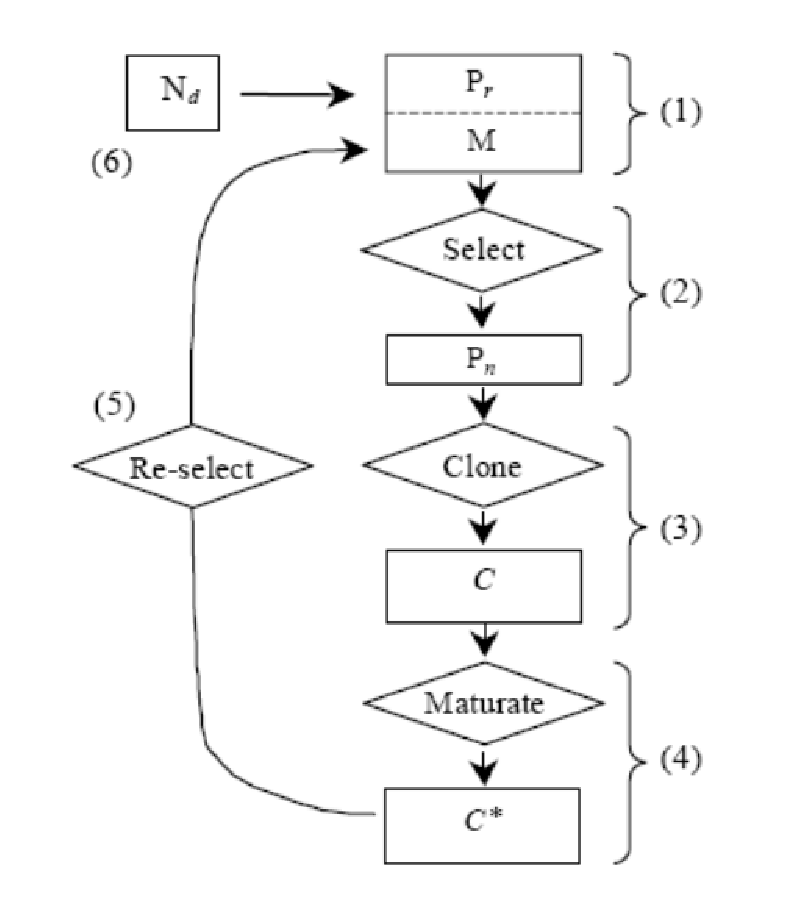
\includegraphics[width=0.5\textwidth]{img/algoritmo}
\end{center}
\caption{Diagrama del algoritmo de la selección clonal}
\label{fig:algoritmo}
\end{figure}

Siendo la explicación de los pasos de la figura~\ref{fig:algoritmo} la siguiente:
\begin{enumerate}
    \item Generar un conjunto (P) de soluciones candidatas, compuesto de células de memoria (M) añadidas a la población restante (Pr), teniendo entonces $P = Pr + M$
    \item Determinar los $n$ mejores individuos (Pn) de la población (P), basado en una medida de afinidad.
    \item Clonar (reproducir) estos $n$ mejores individuos de la población proporcional a su fitness, dando origen a una población temporal de clones (C).
    \item Someter la población de clones a un esquema de hiper-mutación (inversamente proporcional a la afinidad del anticuerpo). Una población de anticuerpos maduros es generada (C*).
    \item Seleccionar nuevamente los mejores individuos de (C*) para componer el conjunto de memoria. (Algunos reemplazos desde (C*) a (P), debido a la mejora)
    \item Reemplazar los $d$ anticuerpos con menor afinidad de la población, manteniendo la diversidad.
\end{enumerate}



\subsection{Estado del Arte Técnica}
%%Descripción de otras experiencias similares a la que se estudiará.
%Esta sección deberá contener la descripción de experiencias con el mismo problema/técnica
%(las mejores) o para problemas similares que puedan ayudarle como refrencia para su propuesta.

Desde que De Castro et al. publicó su trabajo \emph{`` Learning and optimization using clonal selection principle''}~\cite{decastro},
distintos investigadores se han dedicado a poder utilizar dicha teoría para implementar algoritmos que buscan
optimizar una tarea determinada, de hecho, la mayoría de los trabajos se centran en por ejemplo la \emph{optimización
de funciones}, \emph{optimización multiobjetivo}, sin dejar de lado los problemas típicos de optimización como lo son
\emph{path planning}, \emph{graph coloring}, \emph{vehicle routing}, \emph{entrenamiento de sistemas}, \emph{clasificadores},
\emph{reconocimiento de patrones}, etc, pero la presente sección se centra netamente en problemas abordados que puedan
tener una cierta relación a nivel de modelamiento, objetivos o tratamiento con el problema principal del presente trabajo,
el \emph{Car Sequencing Problem}.\\


% Clonal Selection based Mobile Robot Path Planning

Respecto al área de la robótica, Xuanzi Hu~\cite{robotPlanning} a podido dar un enfoque a las problemáticas relacionadas
con el \emph{Mobile Robot Path Planning}, realizando una comparativa con los algoritmos genéticos, en los cuales queda demostrado
la eficiencia y superioridad de la selección clonal, ya que al ser dos metodologías generacionales, se basan en los mismo principios,
y son fácilmente comparables al momento de realizar un \emph{benchmark} de ambas técnicas con parámetros lo más similar posible.
Una característica especial de la presente implementación son sus operadores inmunes utilizados, en los que están el operador de mutación
que consiste en elegir aleatoriamente un nodo del camino y reemplazarlo por otro nodo que no está en el camino original; el operador
de inserción, que se utiliza para poder reparar los segmentos de un camino infactible, insertando un nodo entre el problema y por último
el operador de supresión, que se aplica a los caminos factibles e infactibles. 

Un punto importante en éste trabajo es que a nivel de programación algorítmica, la selección clonal presenta una superioridad también,
al poder ser un algoritmo mucho más sencillo de  implementar que un algoritmo genético.\\
%%


% Scheduling Aircraft Landing Based on Clonal Selection Algorithm and Receding Horizon Control
Por otro lado Xiaolan Jia et al.~\cite{aircraft} utiliza la selección clonal hibridamente en conjunto con un modelo
de control predictivo llamado \emph{Receding Horizon Control (RHC)} para abordar el conocido problema de \emph{Scheduling Aircraft Landing},
en el cual la selección clonal forma parte del algoritmo RHC, ocupándose de realizar el scheduling propiamente tal.

Detalladamente las dos aproximaciones que plantea el presente trabajo de X. Jia, señala que una selección clonal con restricciones
basado en ``grados de infactibilidad'' (IFD) programa los aviones en el \emph{receding horizon} actual, en cambio
el RHC repite el proceso de optimización usando ``propagación de segmentos excelentes de genes'' (EGSS) hasta que todos los aviones
han aterrizado.

IFD maneja las restricciones de una buena manera y guía el proceso de optimización de manera efectiva,
por otro lado EGSS mejora la velocidad de convergencia del algoritmo, demostrando empíricamente que la aproximación con RHC
soluciona el problema de una manera mas efectiva y rápida.\\
%%


% Clonal Selection Algorithm for Vehicle Routing

Otro problema de optimización conocido como \emph{Vehicle Routing Problem (VRP)} ha sido atacado utilizando la selección clonal
también por varios autores, entre ellos destaca Jacek Dabrowski~\cite{vrp} pues soluciona una pequeña variación del
problema en conjunto llamado \emph{Capacitated Vehicle Routing Problem (CVRP)} en el cual una flota fija de vehículos de repartición
con una capacidad uniforme debe atender la demanda de un cliente determinado para un solo producto de un sólo almacén, cumpliendo
obviamente el mínimo costo de transito. Por lo que la única variación entre CVRP y VRP es que el primero añade la restricción
de que todos los vehículos deben tener una capacidad uniforme de un sólo producto.

Dabrowski señala que la selección clonal es una buena herramienta para la búsqueda de caminos múltiples,
ya que cuando entregamos una instancia del programa se puede un conjunto de soluciones como un conjunto de anticuerpo,
rankeando las soluciones mediante ``operadores de comparación'' y pero que existe un control sobre el ``operador de mutación''
entre los cuales están; EXC, que elige esquinas del camino y las trata de unir; SUM, que intenta concatenar dos rutas sin violar
restricciones; NEW, que construye nuevas ruta utilizando la heurística \emph{greedy} a partir de un vértice aleatorio.

Finalmente el único problema es que el autor señala que sería correcto realizar un benchmark con otras técnicas,
para poder comprobar que tan efectiva es la técnica.\\
%%


% Stretching Technique-based Clonal Selection Algorithm for Flexible Job-shop Scheduling
Como ya se vio anteriormente, en muchas investigaciones se utiliza la mezcla entre la selección clona y otra técnica,
y es el mismo casi que propone Lu Hong~\cite{jobshop} al utilizar una técnica de \emph{Stretching} al resolver
una variación del \emph{Job-shop scheduling problem (JSP)} llamado \emph{Flexible Job-shop Scheduling Problem (FJSP)},
la cual solo posee una mayor disponibilidad de máquinas para realizar las operaciones, es decir, sigue la dinámica
de encontrar una ubicación de cada operación y definir las secuencias de éstas en cada máquina, tratando de utilizar el mínimo
tiempo posible.

La técnica de \emph{stretching} fue propuesta por M. N. Vrahatis~\cite{stretching},
%M. Vrahatis, G. Androulakis and M. Manoussakis, “A new unconstrained optimization method for Imprecise function andgradient values,”
%Journal of Mathematical Analysis and Applications, 1996, pp. 586–607.
y su idea principal es realizar dos etapas de transformación sobre la forma de la función objetivo,
basada en la información de los mínimos locales, es decir, si hay un mínimo se busca realizando un algoritmo
de optimización convencional, y cuando se encuentra, la función objetivo se ``estira'' de acuerdo a unas expresiones determinadas.

Utilizando la función de \emph{stretching} no se cambian los objetivos buscando, pero provee una forma de escape
de los óptimos locales mejorando la convergencia global.

Generalmente luego de los test, STCSA muestra ser mejor que una selección clonal normal,
siendo una excelente aproximación para resolver problemas a larga escala cuando otros algoritmos fallan dando buenas soluciones.\\
%%


% Immune Clonal Selection Algorithm for Hybrid Flow-shop Scheduling Problem
Feng Liu et al.~\cite{flowshop} para poder reducir la complejidad computacional del
\emph{Hybrid Flow-shop Scheduling Problem} utiliza selección clonal.

Éste problema es una aplicación importante en las empresas manufactureras, ya que es un problema NP-completo,
y actualmente las tecnologías de optimización y algunas heurísticas como \emph{branch and bound}, \emph{genetic algorithm}
han sido utilizadas pero sin tanto éxito, ya que tienen distintos inconvenientes al momento de trabajar con problemas
de alto tamaño.

Liu realiza ésta elección, pues la selección clonal propone mecanismos especiales como la habilidad de mantener la diversidad
de los anticuerpos, mecanismos de auto-adaptación y funciones de memoria. Además para mejorar la exploración y explotación
se agrupan estrategias y operadores de multi-mutación (mutación clonal, cruzamiento clonal y selección clonal).\\
%%


% Computer Experiments with a Parallel Clonal Selection Algorithm for the Graph Coloring Problem
Finalmente, existen trabajos dignos de destacar, como la aproximación que entrega Jacek Dabrowski~\cite{graph}
al realizar experimentos con selección clonal pero utilizando conceptos de paralelismo para un problema básico como lo es
el \emph{Graph Coloring Problem}, comparandolo contra un algoritmo \emph{Tabu search} en paralelo.

Los anticuerpos son inicializados utilizando una asignación aleatorias de colores o utilizando una heurística \emph{greedy},
por otro lado, la selección clonal se enfoca a minimizar la función objetivo, siendo ésta el numero de conflictos de colores.

El mecanismo de hiper-mutación cambia la asignación de colores a los vértices del gráfico.

Para mejorar el desempeño de la versión paralela que se ha creado se utilizada el modelo de ``isla'' (asincrónico),
donde cada procesador trabaja con su propio conjunto de anticuerpos.

Lo llamativo surge al existir mecanismos de ``migración'' que permite un intercambio de conocimiento entre los 
distintos procesos, los cuales son elegidos mediante una ``selección de torneo''.

Por lo tanto la selección clonal se sobrepone a \emph{Tabu search} en todas las instancias,
llegando a la conclusión que aunque no posea un operador de cruzamiento, la selección clonal
es una forma fácil de implementar un algoritmo de optimización.
%%


Finalmente los algoritmos inmunes, en especial los algoritmos de ``selección clonal'' suelen ser una buena aproximación
para poder solucionar problemas de optimización y gracias a los estudios analizados en el estado del arte del problema,
podemos decir que es una buena solución para el ``Car Sequencing Problem''.


\section{Algoritmo Propuesto}

\subsection{Representación y Función de Evaluación}
\frame
{
\frametitle{Representaciones}
\begin{center}
	\includegraphics[width=0.7\textwidth]{img/representacion}
\end{center}
}

\frame
{
\frametitle{Representaciones}
\framesubtitle{Simulated Annealing}
\begin{itemize}
	\item Variables utilizadas
		\begin{itemize}
			\item {\tt T\_max:} Temperatura máxima.
        	\item {\tt N\_recal:} Número de recalentamientos.
			\item {\tt alpha:} Porcentaje de la temperatura máxima a recalentar.
			\item {\tt Delta\_t:} Temperatura a decrecer, el decrecimiento es aritmético.
			\item {\tt X:} Almacena la solución actual del problema, además se define {\tt x\_gen} y {\tt x\_opt}.
			\item {\tt Delta\_x:} Variación en la función objetivo.
		\end{itemize}
\end{itemize}
}

\frame
{
\frametitle{Representaciones}
\framesubtitle{Simulated Annealing}
\begin{itemize}
	\item Movimiento
	\begin{itemize}
		\item El movimiento escogido es el {\bf swap}, que realiza el cambio de dos variables.
		\item Este cambio se realiza al {\bf azar}, lo que genera una solución que será aceptada bajo las condiciones:
		\begin{itemize}
			\item Si es la función objetivo es menor que la actual, será aceptada.
			\item Si $P(0,1) \leq e^{-|delta_x|}$, será aceptada.
		\end{itemize}
	\end{itemize}
\end{itemize}
}

\begin{frame}[fragile]
\frametitle{Representaciones}
\framesubtitle{Simulated Annealing}
\tiny{
\begin{verbatim}
Inicio
t<-t_max // temperatura inicial
cont <- 0 // número de recalentamientos hechos
Leer Datos
solución<-Generar solución inicial
rest_h<-Contar restricciones violadas de solución
salir<-falso
rest<-rest_h
Mientras cont<numero
    rechazado<-falso
    Mientras rachazado=falso
        solución_gen<- Realizar movimiento a solución
        rest_gen<-Contar restricciones violadas de solución_gen
       	Verifica la aceptación
		Cambiar solución y rest por solución_gen y rest_gen si es mejor o es peor pero se acepta
        Cambiar solución_h y rest_h por solución_gen y rest_gen si es mejor
    Fin Mientras
    Decrecimiento de la temperatura   
    Si t<0 Entonces
        cont<-cont+1
        t<-t*alpha //alpha es una valor entre 0 y 1
    Fin Si
Fin Mientras
Imprimir Resultados
Fin
\end{verbatim}
}
\normalsize
\end{frame}

\frame
{
\frametitle{Representaciones}
\framesubtitle{Algoritmo Evolutivo + Simulated Annealing}
\begin{itemize}
	\item Aproximación a al representación matemática (fórmula).
	\item Estructuras de datos:
	\begin{itemize}
		\item Individuos (\texttt{{\bf struct} genotype}).
		\begin{itemize}
			\item {\tt{\bf int} gene[VARS]}, {\tt {\bf int} fitness}, {\tt {\bf int} fail}.
			\item {\tt {\bf double} rfitness}, {\tt {\bf double} cfitness}.
		\end{itemize}
	\end{itemize}
\end{itemize}
}

\frame
{
\frametitle{Representaciones}
\framesubtitle{Algoritmo Evolutivo + Simulated Annealing}
\begin{itemize}
	\item Estructuras de datos:
	\begin{itemize}
		\item Mejor Solución SA. ({\tt {\bf int} saBestSol[VARS]}).
		\item Número máximo de autos por subsecuencia.\\({\tt {\bf int} numMaxCarOptSeq[N]}).
		\item Tamaño de la subsecuencia. ({\tt {\bf int} sizeMaxCarOptSeq[N]}).
		\item Demanda y descripción de tipos de autos. ({\tt {\bf int} types[N][M]}).
	\end{itemize}
	\item Movimiento SA:
	\begin{itemize}
		\item {\bf swap}
		\item {\tt 10\% VARS}
	\end{itemize}
\end{itemize}
}

\begin{frame}[fragile]
\frametitle{Representaciones}
\framesubtitle{Algoritmo Evolutivo + Simulated Annealing}
\tiny{
\begin{verbatim}
Inicio
g <- 0 & p <- 0 // numero de generaciones y poblaciones
Leer datos de entrada
Población <- Generar población inicial
Evaluar población
    Mientras g < GENS
        Mientras n < POP - 1
            Selección individuo
            Mutación // Simulated Annealing + AM
        Fin Mientras
        Elitismo
        Cambio de población // Población actual = Población nueva
        Evaluar población
        n <- n + 1  &  p <- 0
    Fin Mientras
Imprimir resultados
Fin
\end{verbatim}
}
\normalsize
\end{frame}



\subsection{Algoritmo Propuesto}
Debido a la cantidad de elementos que varían para probar el desempeño
del algoritmo, se ha establecido un conjunto de parámetros que hacen
referencia a la ejecución "base" del algoritmo.
\begin{itemize}
	\item Repertorio Inicial: Arreglado (Cumpliendo restricciones duras).
	\item Selección de Clones: Mejores (Considerando la población actual y la de clones).
	\item Movimiento: Swap al 40\%.
	\item Reemplazo: Peores.
	\item Clonación: Mediante fórmula (explicada más adelante).
\end{itemize}

\begin{enumerate}
	\item \textbf{Repertorio Inicial}

		El repertorio inicial, se ha generado de dos formas para poder establecer una mejor opción.
		\begin{itemize}
			\item \emph{Arreglado:} 
				
				Se ha generado la población inicial con una lista de vehículos que contiene
				la cantidad exacta de los tipos necesitados por el problema, los cuales
				han sido desordenados, para dejar satisfechas en todo momento las restricciones
				blandas.
		\end{itemize}

	\item \textbf{Operador de Selección}
		\begin{itemize}
			\item \emph{Roulette wheel:}
 
				Al momento de seleccionar individuos para realizar la clonación, se utilizó la conocida técnica llamada
				\emph{roulette wheel}, para una Función Objetivo que minimiza.
				
				El procedimiento es bien simple, sólo tenemos que considerar el \emph{fitness} de cada linfocito y calcular un
				\emph{fitness relativo} de la siguiente forma:
				
				$$relativeFitness_{i}\ = \frac{f_{min} + f_{max} - f_{i}}{\sum\limits_{i=0}^{sizePop} (f_{min} + f_{max} - f_{i}}$$
				
				Donde $f_{max}$ equivale al \emph{fitness} del mejor linfocito,
				$f_{min}$ equivale al \emph{fitness} del peor linfocito y
				$f_{i}$ equivale al \emph{fitness} del i-ésimo linfocito de nuestra población.
				
				La suma de todos los \emph{fitness relativo} equivale a $1$.
					
				Luego de que cada linfocito posee su \emph{fitness relativo}, se procede a calcular un \emph{fitness acumulativo},
				es decir, ir sumando las probabilidades para generar un rango entre $0$ y $1$ con todas nuestras probabilidades.
					
				Una vez se tiene el \emph{fitness acumulativo} listo, se procede a obtener un número aleatorio entre $0$ y $1$,
				para que luego sea ubicado en nuestro rango, y así el linfocito que salga escogido con éste número aleatorio, será
				elegido para pasar ahora a la transformación.
		
		\end{itemize}
	\item \textbf{Operador de Clonación}
		\begin{itemize}
			\item \emph{Fórmula:}

				Se ha tomado la esencia de la fórmula propuesta por De Castro~\cite{decastro},
				en el cual consideramos tres elementos: ``factor de clonación ($\beta$)~\footnote{$clonationRate$
				corresponde al tamaño del $40\%$ de la población}'', ``Total de anticuerpos($N$)'' y
				``Afinidad (ranking) ($a$)''.
				La relación está dada por un número $m$ que equivale a la cantidad de clones que se generarán
				para cada anticuerpo ordenados por afinidad, partiendo del mejor al peor.
				$$m\ =\ \lceil\frac{\beta \cdot N}{a}\rceil$$

				Con ésto estamos siguiendo la idea central del algoritmo, pues estamos favoreciendo a que se clonen más
				los mejores elementos de nuestra población.
				
		\end{itemize}
	\item \textbf{Operador de Reemplazo}
		Para mantener la diversidad en nuestra población e intentar escapar de los óptimos locales,
		se utiliza un $replaceRate$ que corresponde a la cantidad del $60\%$ del tamaño de la población.

		Los nuevos elementos son generados cumpliendo las restricciones duras, para obtener nuevos
		elementos un poco mejores en comparación a la creación aleatoria.
		\begin{itemize}
			\item \emph{Peores:}
				Se realiza el reemplazo en los peores elementos de la nueva población a utilizar.

		\end{itemize}
		% Tabla comparativa
	\item \textbf{Movimiento}
		En éste caso se realiza un \emph{swap}, pero como cada individuo es del orden de $200$, $300$ y $400$ autos,
		se realiza una cantidad de \emph{swap} equivalente al $40\%$ de la cantidad de autos.
	
		Para ver que elementos hacen el \emph{swap}, se eligen aleatoriamente dos elementos para intercambiar.
\
\end{enumerate}


Respecto a los gráficos comparativos de cada situación,
se ha realizado 5 configuraciones distintas, para ver la diferencia en el rendimiento:
\begin{enumerate}
    \item Normal:

        \begin{itemize}
            \item Generación de población: Cumpliendo restricciones duras.
            \item Selección de clones: Selección de los mejores.
            \item Reemplazo al término de iteración:  Se reemplazan los peores.
            \item Tipo de clonación: Mediante fórmula.
        \end{itemize}
    \item Población aleatoria:

        \begin{itemize}
            \item Generación de población: \textbf{Rompiendo restricciones duras}.
            \item Selección de clones: Selección de los mejores.
            \item Reemplazo al término de iteración:  Se reemplazan los peores.
            \item Tipo de clonación: Mediante fórmula.
        \end{itemize}

    \item Selección ruleta:

        \begin{itemize}
            \item Generación de población: Cumpliendo restricciones duras.
            \item Selección de clones: \textbf{Selección mediante ruleta}.
            \item Reemplazo al término de iteración:  Se reemplazan los peores.
            \item Tipo de clonación: Mediante fórmula.
        \end{itemize}

    \item Reemplazo aleatorio:

        \begin{itemize}
            \item Generación de población: Cumpliendo restricciones duras.
            \item Selección de clones: Selección de los mejores.
            \item Reemplazo al término de iteración:  \textbf{Se reemplazan aleatoriamente}.
            \item Tipo de clonación: Mediante fórmula.
        \end{itemize}

    \item Secuencia Fija:

        \begin{itemize}
            \item Generación de población: Cumpliendo restricciones duras.
            \item Selección de clones: Selección de los mejores.
            \item Reemplazo al término de iteración:  Se reemplazan los peores.
            \item Tipo de clonación: \textbf{Secuencia fija}.
        \end{itemize}

\end{enumerate}

Los resultados obtenidos y graficados corresponden al \emph{promedio}, \emph{desviación estándar},
\emph{valores mínimos}, \emph{valores máximos} y \emph{tiempo de ejecución}.


Ver anexo~\ref{sec:anexo}.


\begin{frame}[fragile]
\frametitle{Algoritmo}
\tiny
\begin{verbatim}
    Inicio
    g <- 0 // numero de generaciones
    Leer datos de entrada
    Población <- Generar población inicial
    Evaluar población

    Mientras g < GENS
        Limpiar poblaciones
        Seleccionar individuos a clonal (ruleta)
        Clonación (fórmula)
        Hipermutación mediante Swap
        Evaluar población mutada
        Selección de clones (Mejores)
        Inserción de clones en nueva población
        Generar elementos nuevos aleatorios
        Inserción de elementos nuevos al población
        g <- g + 1
    Fin Mientras

    Imprimir resultados
    Fin
\end{verbatim}
\end{frame}



\section{Sintonización}

\subsection{Parámetros}
%Definición y análisis de cada uno de los parámetros que posea su algoritmo. \\
%
%Ej. \textit{Temperatura (Simulated Annealing); [0,1] parámetro que define la probabilidad con la cual se aceptan soluciones de peor calidad en cada iteración. Un valor alto para este parámetro involucra una fuerte e exploración, en cambio valores bajos indican una inclinación a la explotación.} \\
%Puede incluir diagramas o todo lo que sea necesario para dejar claras las caracteristicas y función que cumple el parámetro en su algoritmo.

\begin{itemize}
	\item \texttt{POP} \blue{(20)}, Parámetro que define el tamaño de cada población al momento de comenzar
			las iteraciones a través de la cantidad de generaciones.
			Este parámetros influye notablemente en el tiempo que demora la ejecución de nuestro algoritmo,
			pues si tenemos poblaciones muy grandes todo el tratamiento que le damos a los individuos,
			como la hipermutación y la clonación tomará mucho más tiempo.
	\item \texttt{GENS} \blue{(200)}, Parámetro que define el número total de generaciones en las cuales
			el algoritmo se mantendrá en ejecución. Este parámetro es la actual condición de término
			por lo cual es escencial a la hora de obtener buenos o malos resultados, ya que si tenemos
			muy pocas generaciones, para muchas variables puede que no se alcance a cumplir bien los
			objetivos del algoritmo y que se termine no con los mejores resultados.
	\item \texttt{selRate} POP*0.4  // Tasa para la cantidad de elementos seleccionados
	\item \texttt{swap} VARS*0.4 // Cantidad de swap realizados en el movimiento
	\item \texttt{mutRate} POP*0.02

	\item \texttt{clonationFactor} = 0.0;//0.5 // Factor para calcular individuos clonados
	\item \texttt{clonationRate} = 0.0; //POP*0.4 // Tasa para realizar la clonación
	\item \texttt{replaceRate} =  0.0; //POP*0.6  // Tasa para la cantidad de elementos reemplazados
\end{itemize}


\subsection{Pruebas de sintonización}
\subsubsection{Sintonización Manual}
%Se deben explicar todas las pruebas de sintonización manual realizadas. Para esto debe usar la estructura que se adjunta abajo.\\

Para la presente sección, se requiere de una configuración inicial,
para poder comenzar a evaluar el rendimiento del algoritmo para
cada situación donde se quiera sintonizar manualmente algún parametro.

Los valores de la configuración inicial están dado en base a la experiencia
del trabajo pasado, es decir, en la \emph{primera implementación}.

\begin{itemize}
	\item \texttt{POP = 20}
	\item \texttt{GENS = 200}
	\item \texttt{clonationFactor = 0.4}
	\item \texttt{clonationRate = 0.5}
	\item \texttt{replaceRate = 0.6}
\end{itemize}

Complementariamente, se han considerado tres instancias provenientes de la CSPlib~\cite{CSP}
más precisamente de la sección \emph{``30 new hard problems from Caroline Gagne ''},
donde se han escogido tomando en cuenta el mejor resultado encontrado.
Las instancias son:

\begin{center}
	\begin{tabular}{|l|c|}
	\hline
	\textbf{Instancia} & \textbf{Mejor resultado conocido} \\\hline
	\texttt{pb\_200\_01.txt} & 0 \\\hline
	\texttt{pb\_200\_09.txt} & 10 \\\hline
	\texttt{pb\_200\_10.txt} & 19 \\\hline
	\end{tabular}
\end{center}
\newpage
\subsubsection{Tamaño de población}

\textbf{Prueba}: \blue{prueba1}\\

\textbf{Parámetros involucrados:} Tamaño de población \texttt{(POP)}.\\

\textbf{Objetivo:} Analizar el comportamiento de acuerdo a fitness y tiempo de ejecución del parámetro en un rango de valores.\\

\textbf{Metodología:} Se probarán varios valores en el rango de valores del parámetro \blue{[10,210]}.\\

\textbf{Gráfico:}\\

\begin{figure}[h!]
\begin{center}
	\includegraphics[width=0.95\textwidth]{img/1.pdf}
	\caption{Comparaci\'on de las tres instancias dado un cambio en la poblaci\'on}
	\label{fig:1}
\end{center}
\end{figure}

\textbf{Configuración escogida:}\\

\begin{center}
\begin{tabular}{|l|c|c|c|c|}
	\hline
	\textbf{Instancia} & \textbf{POP} & \textbf{Mejor resultado} & \textbf{Tiempo [s] } & \textbf{Tiempo total [s] }\\\hline
	\texttt{pb\_200\_01.txt} & 195 & 167 & 15.110 & 1608.853 \\\hline 
	\texttt{pb\_200\_09.txt} & 150 & 152 & 11.243 & 1593.739 \\\hline
	\texttt{pb\_200\_10.txt} & 158 & 126 & 11.210 & 1662.580 \\\hline
\end{tabular}
\end{center}

\newpage
\subsubsection{Número de generaciones}

\textbf{Prueba}: \blue{prueba2}\\

\textbf{Parámetros involucrados:} Número de generaciones \texttt{(GENS)}.\\

\textbf{Objetivo:} Analizar el comportamiento de acuerdo a fitness y tiempo de ejecución del número de generaciones entre un rango de valores.\\

\textbf{Metodología:} Se probarán varios valores en el rango de valores del parámetro \blue{[10,2000]} (iterando de 30 en 30).\\

\textbf{Gráfico:}\\

\begin{figure}[h!]
\begin{center}
	\includegraphics[width=0.95\textwidth]{img/2.pdf}
	\caption{Comparaci\'on de las tres instancias dado un cambio en el n\'umero de generaciones}
	\label{fig:2}
\end{center}
\end{figure}

\textbf{Configuración escogida:}\\

\begin{center}
\begin{tabular}{|l|c|c|c|c|}
	\hline
	\textbf{Instancia} & \textbf{GENS} &\textbf{Mejor resultado} & \textbf{Tiempo [s] } & \textbf{Tiempo total [s]}\\\hline
	\texttt{pb\_200\_01.txt} & 1810 & 186 & 7.782 & 256.177 \\\hline
	\texttt{pb\_200\_09.txt} & 1960 & 166 & 8.460 & 262.906 \\\hline
	\texttt{pb\_200\_10.txt} & 1630 & 144 & 7.562 & 256.546 \\\hline
\end{tabular}
\end{center}

\newpage
\subsubsection{Tasa de reemplazo}

\textbf{Prueba}: \blue{prueba3}\\

\textbf{Parámetros involucrados:} Tasa de reemplazo \texttt{(replaceRate)}.\\

\textbf{Objetivo:} Analizar el comportamiento de acuerdo a fitness y tiempo de ejecución de la tasa de reemplazo entre un rango de valores.\\

\textbf{Metodología:} Se probarán varios valores en el rango de valores del parámetro \blue{[0,1]}.
Para éste caso en particular, se ejecutó el algoritmo 10 veces por cada valor del parámetros y luego se seleccionó la mejor
para poder hacer el siguiente análisis.\\

\textbf{Gráfico:}\\

\begin{figure}[h!]
\begin{center}
	\includegraphics[width=0.95\textwidth]{img/3.pdf}
	\caption{Comparaci\'on de las tres instancias dado un cambio en la tasa de reemplazo}
	\label{fig:3}
\end{center}
\end{figure}

\textbf{Configuración escogida:}\\

\begin{center}
\begin{tabular}{|l|c|c|c|c|}
	\hline
	\textbf{Instancia} & \textbf{POP*replaceRate} & \textbf{Mejor resultado} & \textbf{Tiempo [s]} & \textbf{Tiempo total [s]}\\\hline
	\texttt{pb\_200\_01.txt} & 8 & 200 & 1.374 & 13.246 \\\hline
	\texttt{pb\_200\_09.txt} & 0 & 178 & 1.463 & 12.027 \\\hline
	\texttt{pb\_200\_10.txt} & 0 & 164 & 0.515 & 12.133   \\\hline
\end{tabular}
\end{center}


\newpage
\subsubsection{Factor de clonación y Tasa de clonación}

\textbf{Prueba}: \blue{prueba4} \\

\textbf{Parámetros involucrados}: Tasa de clonación y Factor de clonación. \\

\textbf{Objetivo}: Estudiar el efecto de la tasa y el factor de clonación en conjunto de acuerdo a fitness obtenido para la variación
de los dos parámetros en todo tu dominio.\\

\textbf{Metodología}: Se prueban varias combinaciones de valores para ver el efecto de los parámetros y poder observar su comportamienteo.\\

\textbf{Configuración escogida:}\\

\begin{small}
\begin{center}
\begin{tabular}{|l|c|c|c|c|c|}
	\hline
	\textbf{Instancia} & \textbf{clonationRate} & \textbf{clonationFactor} &\textbf{Mejor resultado} & \textbf{Tiempo [s]} & \textbf{Tiempo total [s]}\\\hline
	\texttt{pb\_200\_01.txt} & 0.6 & 1   & 192 & 1.241 & 132.608 \\\hline
	\texttt{pb\_200\_09.txt} & 0.6 & 1   & 180 & 1.378 & 132.068 \\\hline
	\texttt{pb\_200\_10.txt} & 0.5 & 0.9 & 160 & 1.379 & 132.124 \\\hline
\end{tabular}
\end{center}
\end{small}
\normalsize
\textbf{Gráfico:}\\

\begin{figure}[h!]
\begin{center}
	\includegraphics[width=0.95\textwidth]{img/01-4.pdf}
	\caption{Comparaci\'on de la instancia \texttt{pb\_200\_01.txt} variando \texttt{clonationRate} y \texttt{clonationFactor}}
	\label{fig:4-1}
\end{center}
\end{figure}

\begin{figure}[h!]
\begin{center}
	\includegraphics[width=0.95\textwidth]{img/09-4.pdf}
	\caption{Comparaci\'on de la instancia \texttt{pb\_200\_09.txt} variando \texttt{clonationRate} y \texttt{clonationFactor}}
	\label{fig:4-2}
\end{center}
\end{figure}

\newpage 
\begin{figure}[h!]
\begin{center}
	\includegraphics[width=0.95\textwidth]{img/10-4.pdf}
	\caption{Comparaci\'on de la instancia \texttt{pb\_200\_10.txt} variando \texttt{clonationRate} y \texttt{clonationFactor}}
	\label{fig:4-3}
\end{center}
\end{figure}


\newpage
%
%
%elegir una configuración para cada instancia
%	-indicar el fitness
%	-identificar claramente las características del algoritmo.
%	-estimación del tiempo en realizarla.

\subsubsection{Sintonización Automática}
%Debe identificar el algoritmo sintonizador que elegirá y los parámetros que serán sintonizados por éste. Utilize la siguiente estructura: \\ \\
%\textbf{Sintonizador}: \\
%\textbf{Parámetros a Sintonizar}:\\
%\textbf{Detalles del sintonizador}: Todo lo que tenga que ver con la configuración usada del sintonizador (veáse en la materia los parámetros de cada sintonizador: iteraciones, individuos, tiempo, tipo de busqueda... etc.)\\ 
%
%Debe finalmente entregar el resultado del sintonizador para cada instancia analizada, junto con el resultado (fitness) de la ejecución del algoritmo con estos parámetros.

\section{Control de Parámetros}
\frame
{
\frametitle{Control de Parámetros}
\framesubtitle{Configuración del problema}
\begin{itemize}
    \item \texttt{POP = 160}
    \item \texttt{GENS = 2000}
    \item \texttt{clonationFactor = 0.8}
    \item \texttt{clonationRate = 0.8}
    \item \texttt{replaceRate = 0.5}
\end{itemize}

}

\frame
{
\frametitle{Control de Parámetros}
\framesubtitle{Cambios}
\begin{itemize}
	\item Semilla de números aleatorios.
	\item Promedio del fitness de un población.
	\item Mejor individuo de cada población.
	\item Diferencias.
\end{itemize}
}
\frame
{
\frametitle{Control de Parámetros}
\framesubtitle{Comportamiento}
\begin{center}
\small{
\begin{tabular}{|l|c|c|c|c|c|c|c|c|}
\hline
  & \multicolumn{3}{|c|}{\textbf{$\Delta$ promedios}} & \multicolumn{3}{|c|}{\textbf{$\Delta$ mejores}} & & \\\hline
\textbf{Instancia} & $+\Delta$ & $0$ & $-\Delta$ & $+\Delta$ & $0$ & $-\Delta$ & \textbf{Fitness} & \textbf{Tiempo} \\\hline
\texttt{pb\_200\_01.txt} & 0 & 0 & 2000 & 1624 & 289 & 87 & 77 & 104.451 \\\hline
\texttt{pb\_200\_09.txt} & 0 & 0 & 2000 & 1605 & 324 & 71 & 71 & 104.833 \\\hline
\texttt{pb\_200\_10.txt} & 0 & 0 & 2000 & 1442 & 486 & 72 & 55 & 102.377 \\\hline
\end{tabular}
}
\end{center}
}
\frame
{
\frametitle{Control de Parámetros}
\framesubtitle{Comportamiento}
\begin{itemize}
	\item Diferencia de promedios negativa $\rightarrow$ Mejores clones.
	\item Diferenci de mejores $\rightarrow$
	\begin{itemize}
		\item Positivas, peores individuos.
		\item Cero, iguales individuos.
		\item Negativas, mejores individuos.
	\end{itemize}
\end{itemize}
}

\frame
{
\frametitle{Control de Parámetros}
\framesubtitle{Primer control}
\begin{itemize}
	\item Parámetros a controlar.
	\begin{itemize}
		\item Tasa de reemplazo (\texttt{replaceRate}) \blue{[0,1]}. 
	\end{itemize}
	\item Gatillador de cambio.
	\begin{itemize}
		\item Diferencia entre los mejores individuos.
	\end{itemize}
	\item Velocidad y mecanismo de cambio.
	\begin{itemize}
		\item Acumulación del $0.2\% GENS$
	\end{itemize}
\end{itemize}
}

\begin{frame}[t,fragile]
\frametitle{Control de Parámetros}
\framesubtitle{Primer control}
\begin{itemize}
	\item Pseudocódigo.
\tiny{
\begin{alltt}
    Inicio
    ...
    Mientras g < GENS
        Limpiar poblaciones
        \blue{Guardar mejor individuo de la población}
        Seleccionar individuos a clonal (ruleta)
        ...
        Selección de clones (Mejores)
        \blue{Guardar mejor individuo de los clones
        Calcular diferencia entre mejores individuos
        Si diferencia < 0
            aumentar contadorA
            Si contador = 0.2\% GENS
               Tasa de reemplazo = Tasa de reemplazo - 10\% POP
               contadorA = 0
        O Sino diferencia > 0
            aumentar contadorB
            Si contadorB = 0.2\% GENS y Tasa de reemplazo < 90\%POP
                Tasa de reemplazo = Tasa de reemplazo + 10\% POP
                contadorB = 0
        O Sino diferencia = 0
            Tasa de reemplazo = 50\% POP
            contadorA = 0
            contadorB = 0
        }
        Inserción de clones en nueva población
        ...
    Fin
\end{alltt}
}
\end{itemize}
\end{frame}

\frame
{
\frametitle{Control de Parámetros}
\framesubtitle{Segundo control}
Basado en ``Homeostatic Regulation of CLONALG with online Parameters Calibration''
\begin{itemize}
	\item Parámetros a controlar.
	\begin{itemize}
		\item Control de clonación (\texttt{clonation\_control}) \blue{[-90\% POP, 90\% POP]}
		\item Tasa de clonacion (\texttt{clonationRate}) \blue{[0,1]} 
	\end{itemize}
	\item Gatillador de cambio.
	\begin{itemize}
		\item Diferencia entre promedios de individuos.
		\item Diferencia entre mejores individuos.
	\end{itemize}
	\item Velocidad y mecanismo de cambio.
	\begin{itemize}
		\item Aumento de control de clonacion (1) si diferencia entre mejores es negativa y viceversa.
		\item Disminuir la tasa de clonación (1) si diferencia entre mejores negativa y promedios positiva.
		\item Controlando límites.
	\end{itemize}
\end{itemize}
}

\begin{frame}[t,fragile]
\frametitle{Control de Parámetros}
\framesubtitle{Segundo control}
\begin{itemize}
	\item Pseudocódigo:
\tiny{
\begin{alltt}
    Inicio
	...
    Mientras g < GENS
        Limpiar poblaciones
        \blue{Obtener mejor individuo de la población
        Obtener el promedio de los fitness de la población}
        Seleccionar individuos a clonal (ruleta)
		...
        Selección de clones (Mejores)
        \blue{Obtener mejor individuo de los clones
        Obtener el promedio de los fitness de los clones
        Calcular diferencia1 entre mejores individuos
        Calcular diferencia2 entre los promedios

        Si diferencia1 < 0 y control clonacion < 10\% POP
            control clonacion ++
        O Sino diferencia1 > 0 y control  clonacion > - 10\% POP
            control clonacion --

        Si diferencia1 < 0 y diferencia2 > 0 y Tasa de clonacion > 2
            Tasa de clonacion --
        O Sino Tasa de clonacion < 90\% POP
            Tasa de clonacion ++
        }
        Inserción de clones en nueva población
		...
    Fin
\end{alltt}
}
\end{itemize}
\end{frame}


\frame
{
\frametitle{Control de Parámetros}
\framesubtitle{Resultados Control}
\begin{center}
\footnotesize{
\begin{tabular}{|l|c|c|c|c|c|c|}
\hline
 & \multicolumn{2}{|c|}{Sin Control} & \multicolumn{2}{|c|}{1er Control} & \multicolumn{2}{|c|}{2do Control} \\\hline
\textbf{Instancias} & \textbf{Fitness} & \textbf{Tiempo} & \textbf{Fitness} & \textbf{Tiempo} & \textbf{Fitness} & \textbf{Tiempo} \\\hline
\texttt{pb\_200\_01.txt} & 77 & 104.734 & \red{75} & 101.152 & 76 & 105.692 \\ \hline
\texttt{pb\_200\_09.txt} & 71 & 104.156 & 66 & 102.252 & \red{64} & 104.641 \\ \hline
\texttt{pb\_200\_10.txt} & \red{55} & 103.314 & 63 & 102.146 & 63 & 105.684 \\ \hline
\end{tabular}
}
\end{center}

}


\section{Resultados Generales}
\frame
{
\frametitle{Resultado}
\framesubtitle{}
\begin{itemize}
	\item tabla y grafico
\end{itemize}
}


\section{Conclusiones}
%Conclusiones revelantes del estudio realizado.

En el presente informe se ha dado un estado del arte de un problema muy popular
en el área de la inteligencia artificial, el \emph{Car Sequencing Problem}, siendo éste
una variación de otro problema connotado llamado \emph{Job Shop Scheduling}.
Es tanto la importancia del presente problema, que la \emph{French Society of Operations
Research and Decision-Making Aid} ha decidido ya hace varios años, comenzar lo que se denomina
\emph{The ROADEF challenge} cada dos años, teniendo como objetivo central,  permitir a las personas
que se desarrollan en el área de la industria el presenciar todos los avances y evoluciones
en el ámbito de la Investigación de Operaciones y Análisis de Decisiones, pero no sólo eso
sino el poder enfrentar directamente problemas decisionales complejos, que ocurren en la industria.
Siguiendo la idea anterior, lo importante de éste \emph{Challenge} es que en el 2005, se consideró
como tema principal el \emph{Car Sequencing Problem} debido a la propuesta que realizó RENAULT,
por lo cual uno podrá imaginar la cantidad de avances que se produjeron, pues cada participante
abordaba el problema desde una metodología distinta.

Por otra parte, pareciera que un problema relacionado a \emph{ordenar} un conjunto de vehículos
para ser ensamblados y así obtener el orden más óptimo, no es una tarea difícil, pero claramente
debido a la complejidad que otorgan las restricciones y de que es un problema de la vida real,
presenta un grado de dificultad mayor, lo cual queda reflejado por la cantidad de publicaciones 
e investigaciones que hay al respecto.

Se dieron a conocer también, tres áreas para atacar el presente problema.
Por un lado tenemos los métodos heurísticos que como bien sabemos, es prácticamente jugar a la ruleta
rusa con nuestra investigación, pues la heurística solamente selecciona un objetivo de los dos provenientes
de la definición, una buena solución o un buen tiempo de ejecución. Pero también se presenta que la heurística
es un mecanismo confiable para decidir \emph{utilizarlo} como un apoyo, mas que utilizarlo solo.

Siguiendo con los mecanismos planteados, se vieron también los  métodos exactos,
es decir, técnicas de optimización, donde podemos encontrar la \emph{programación lineal entera},
\emph{branch and bound} y \emph{local search}, los cuales se dedicaban netamente a construir una
solución óptima a partir de los datos que el mismo problema nos entrega. El único problema que tienen
éstas técnicas es que la complejidad temporal va a crecer demasiado con respecto al tamaño de nuestro
\emph{input} del algoritmo.

Dentro de toda la lectura realizada para las distintas técnicas, pude percatarme que las mejores soluciones
siempre son variaciones de métodos o tomar dos técnicas como complementarias, por ejemplo uno de los
mejores resultados fue la combinación de un \emph{Ant Colony Optimization} con una heurística dinámica,
pues claramente se nos señala que el buen uso de una heurística es crucial, es decir, hay que preocuparse
de leer los estudios que se han publicado, par ver cual es la combinación más óptima.

Finalmente, es impresionante la cantidad de estudios con respecto a éste problema en particular,
por lo que podemos darnos cuenta que muchos centros de investigación han dedicado tiempo valioso
para la resolución óptima del \emph{Car Sequencing Problem}, pero no tanto la versión que se estudió,
que es la propuesta por Parello~\cite{parello}, sino mas bien al desafío de la ROADEF.


\end{document}
